\icode{E-MD-CA-L2-261111-003}
如图所示，质量 \(M =\) \,\qty{3}{kg}、长 \(L =\) \,\qty{2}{m}的薄木板静置在光滑水平地面上，质量 \(m =\) \,\qty{1}{kg}的小滑块（可视为质点）以速度 \(v_0\)从木板的左端水平冲上木板，滑块恰好可以从木板上滑下，已知滑块与木板间的动摩擦因数 \(\mu = 0.3\)，\(g\) 取\qty{10}{m/s^2}。求：
\begin{enumerate}
	\item 滑块的加速度\(a_1\)和薄木板的加速度\(a_2\)；
	\item 滑块的初速度\(v_0\) 的大小；
\end{enumerate}

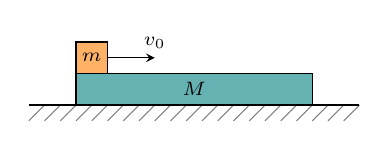
\begin{tikzpicture}[>=stealth,font=\scriptsize]
	\draw[fill=orange!60] (0,.4) rectangle(.4,.8)node[midway]{\(m\)};
	\draw[fill=teal!60] (0,0) rectangle(3,.4)node[midway]{\(M\)};
	\draw[->] (.4,.6)--++(.6,0)node[above]{\(v_0\)};
	\foreach \x in {-.6,-.4,...,3.6}
		\draw[gray] (\x,-.2)--++(.2,.2);
	\draw[thick] (-.6,0)--(3.6,0);
\end{tikzpicture}
\begin{answer}
	（1）\qty{3}{m/s^2}\quad\qty{1}{m/s^2}（2）\qty{4}{m/s^2}
\end{answer}